\chapter{TBtools}

\section{TBtools简介}

(a Toolkitfor Biologists integrating various biological data-handling tools),
是一款集成了blast、KEGG等模块的生信分析软件(软件包主页\textit{https://github.com/CJ-Chen/TBtools/releases}).

TBtools有共130余种不同功能,是一款强大的生信分析-可视化软件。

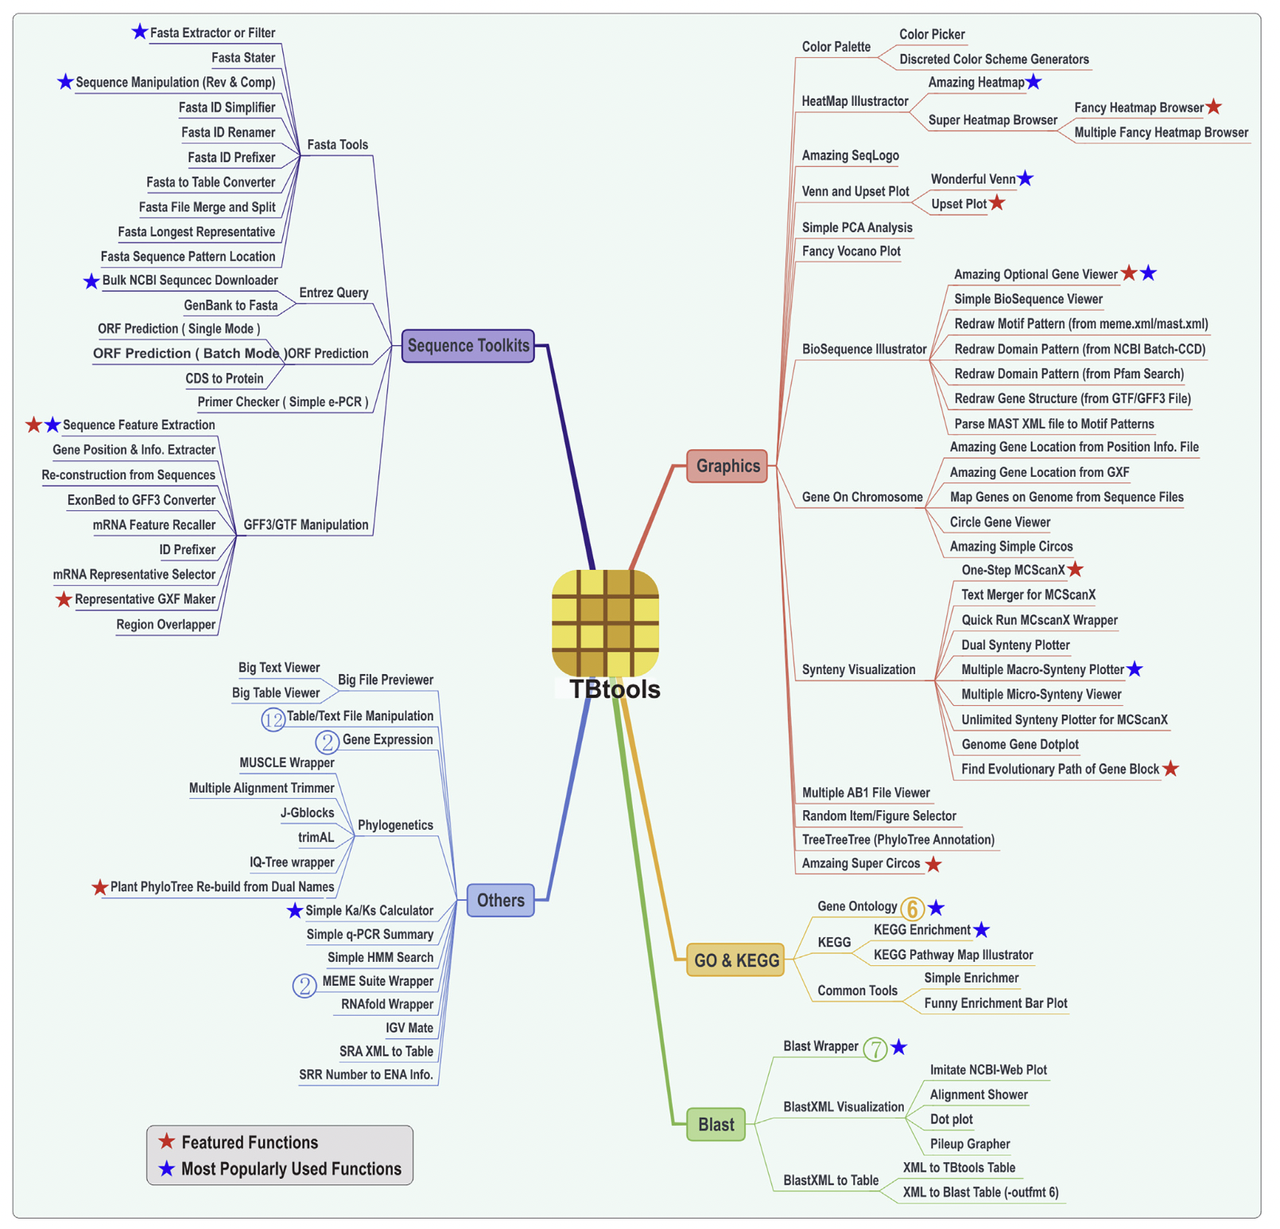
\includegraphics[width=0.8\textwidth]{./image/gdk/8.1.1.png}

\begin{quotation}
    功能总览,图源:https://www.yuque.com/cjchen/hirv8i
\end{quotation}

TBtools是为交互式数据表示而开发的,而数据可视化和表示是生物信息分析不可或缺的部分。与通常生成不可编辑图形的常规图形生成器不同,TBtools生成充满可编辑特征的交互图形。TBtools中集成了一个名为“JIGplot”(Java交互式图形)的新开发的绘图引擎,可以快速修改各种图形功能。

例如:可以在control panel上快速的调节绘画时的各种参数,修改生成的可视化图片,为用户提供了很大的方便性。

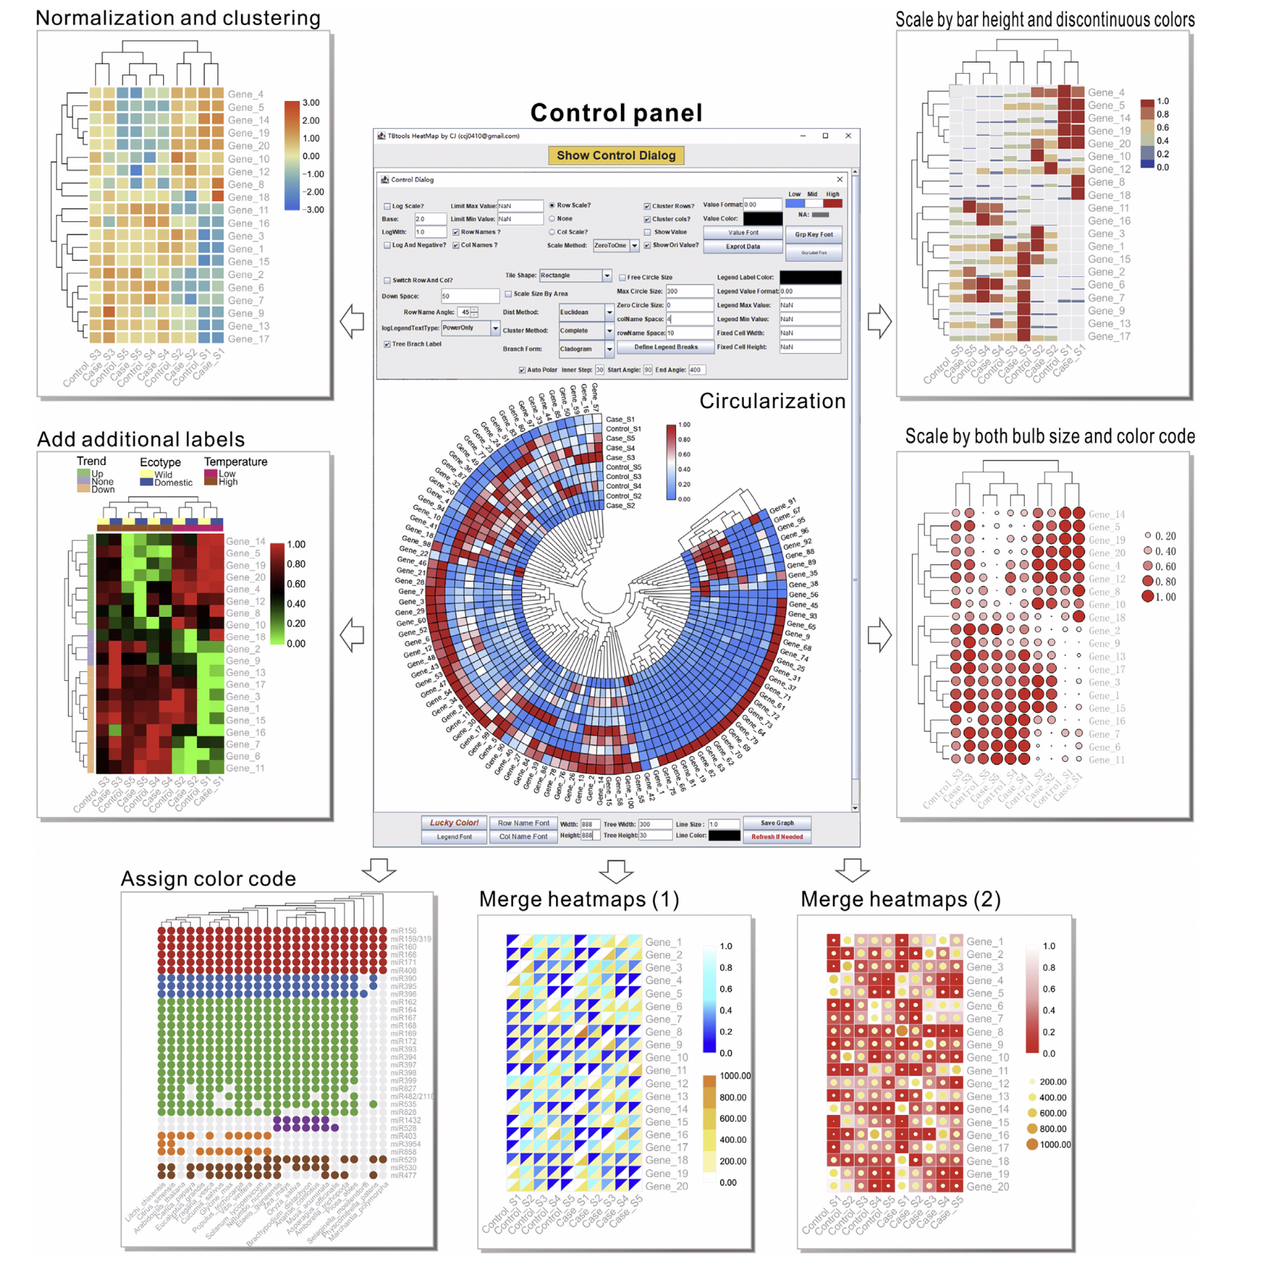
\includegraphics[width=0.8\textwidth]{./image/gdk/8.1.2.png}

本小节中,只对TBtools的功能进行简要介绍,不包含详细的案例分析。

\section{软件功能实例}

\subsection{ORF预测}
\subsubsection{背景}
预测ORF(Open Reading Frame)时,从mRNA角度(起始密码子,canonical或non-canonical等),蛋白质角度(蛋白产物稳定性、是否具有功能等)进行预测。
\subsubsection{常用的ORF预测软件——OrfM}
以往寻找终止密码子的方式:将原始序列切成6种不同的frame,逐个扫描获得终止密码子。

OrfM(\href{https://security.feishu.cn/link/safety?target=https%3A%2F%2Facademic.oup.com%2Fbioinformatics%2Farticle%2F32%2F17%2F2702%2F2450737&scene=ccm&logParams=%7B%22location%22%3A%22ccm_docs%22%7D&lang=zh-CN}{fast open reading frame predictor for metagenomic data})
直接在原始的核苷酸序列种寻找终止密码子,使用Aho-Corasick算法

Aho-Corasick:

    A. 根据已有的数据建立有限的目标pattern和模式匹配机
    B. 使用模式匹配机对文本字符串进行单遍处理。

构建模式匹配机所需的时间与pattern长度的总和成正比。

模式匹配机在处理文本字符串时进行状态转换的次数与关键字的数量无关。

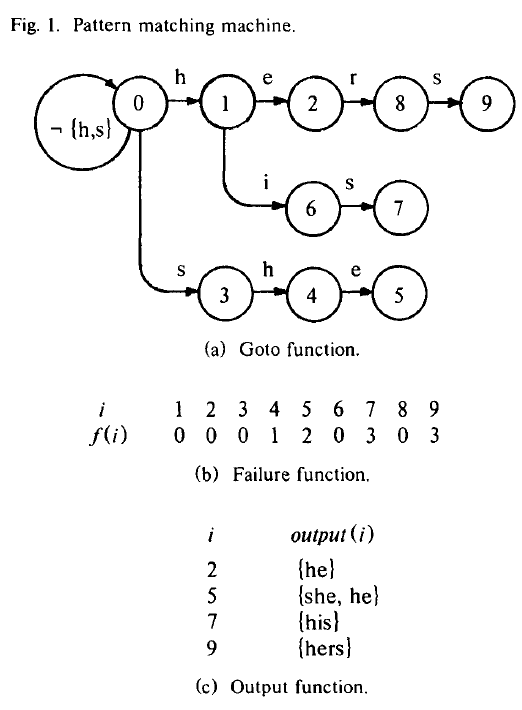
\includegraphics[width=0.6\textwidth]{./image/gdk/8.2.1.png}
\subsubsection{TBtools中的ORF prediction}
可进行单条序列中ORF的预测

批量序列中ORF的预测

批量CDS对蛋白质的转化(是否考虑密码子偏好性)



\subsection{基因富集分析}
\subsubsection{背景}
GO(gene ontology,基因本体论)的主要目的是归类,统一生物学方言(不同的生物学数据库可能会使用不同的术语)。

GO是一个有向无环图(DAG)本体,主要形式是term标记,每个GO term代表一种功能描述,都属于ontology。

GO总共分成三个ontology:molecular function(MF), cellular component(CC)和biological process(BP)。

不同GO term之间存在多种关系,常见的主要是is\_a和part\_of和两种关系.

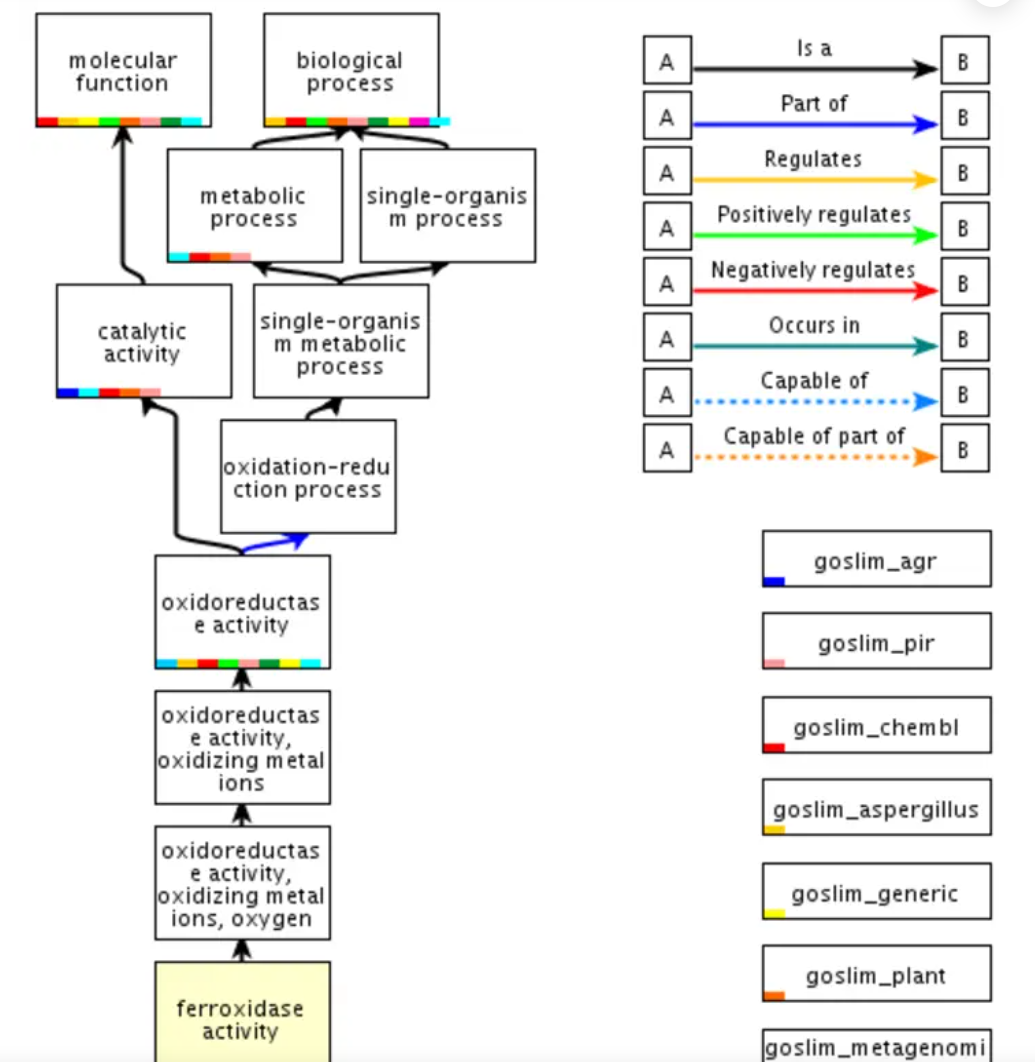
\includegraphics[width=0.75\textwidth]{./image/gdk/8.2.2.png}

\subsubsection{基本原理介绍}
如已有一基因集合(如差异表达基因集合或ChIP-seq的Peaks或GWAS定位的系列区间),
及有一个功能标签(例如如生长素信号转导相关 )。

假定某物种共有100个基因,其中20个基因与生长素信号转导相关,80个基因未注释到与生长素信号转导相关(在该注释库下被认为于无关)。
对植株进行处理,通过差异表达分析鉴定到10个差异表达基因,其中2个与生长素信号转导相关,而另外8个则没注释到生长素信号转导相关。

结果如下:

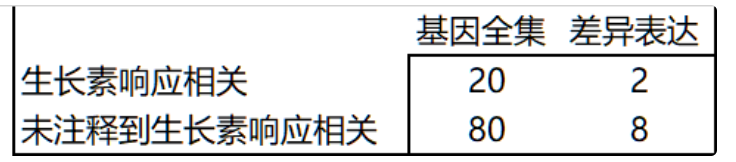
\includegraphics[width=0.8\textwidth]{./image/gdk/8.2.3.png}

检测结果中用于差异分析的基因集合中与生长素相应相关的基因比例与基因全集中与生长素相应相关的基因比例(背景比例相同),说明没有富集。

\begin{quotation}
    注意:

    1. 区别“富集”和“富集显著”:上述按理,若实验组基因集合中具有感兴趣标签的基因的比例超过背景比例,那么这种情况类比上,就是“富集”,因为偏离了背景。但是通过检验,如果偏离程度不大,则不能排除这是一种随机波动;而如果显著偏离了背景分布,就是“富集显著”。
    
    2. 富集分析时,很多新接触的,搞错的往往就是没搞清楚原理,背景(基因全集) 和 实验组基因集合(基因选择集合)(如差异表达基因集合)。一定要注意,做基因功能富集分析是,背景注释指的是这个物种所有基因的功能注释信息而不是选择集的基因功能注释。比如,做拟南芥的,大概有2w+个基因的功能注释,拿这个做背景;而不是拿差异表达的几百上千个基因的注释做背景。
\end{quotation}

\subsubsection{TBtools实现GO富集分析}

需要准备三个文件:

a. go-basic.obo 文件,可以从http://purl.obolibrary.org/obo/go/go-basic.obo下载

b. 一个物种所有基因的GO注释文件

c. 一个基因选择集合,如实验组基因集合,如差异基因集合,或GWAS筛选出来的基因集合等

具体实现过程:

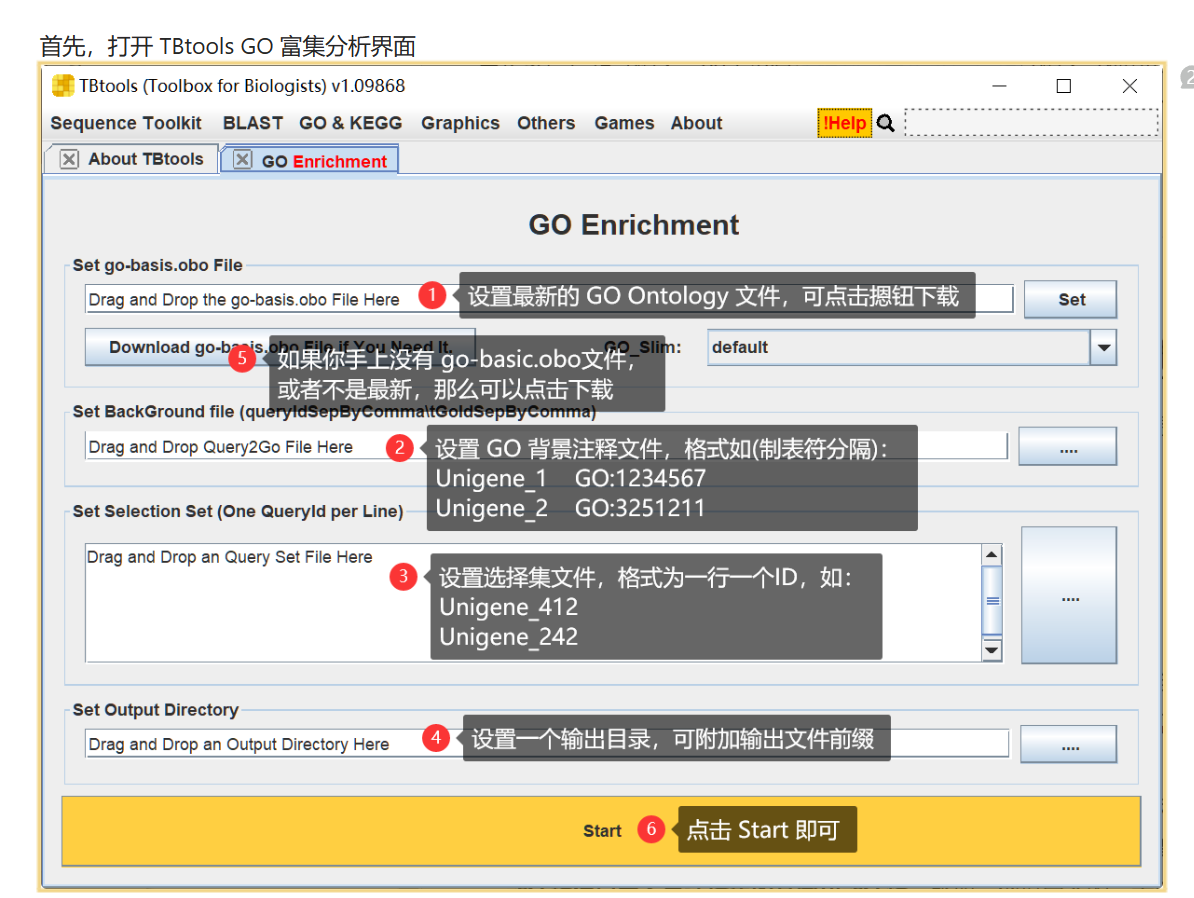
\includegraphics[width=0.8\textwidth]{./image/gdk/8.2.4.png}

\subsection{其他常见功能}

(1)eFP Browser 能够提供一个很简单便捷的方法用来可视化基因在宏观结构上的表达情况

(2)interactive heatmap:提供基因互作关系的程度关系

(3)simple circos:一种常见的基因比较分析可视化方法

......

\subsection{TBtools插件安装}

TBtools的插件模式允许用户在 TBtools 核心功能外按照自己需要安装特定插件,从而使用对应功能。这些插件可以直接在 TBtools 的 插件商店中找到。

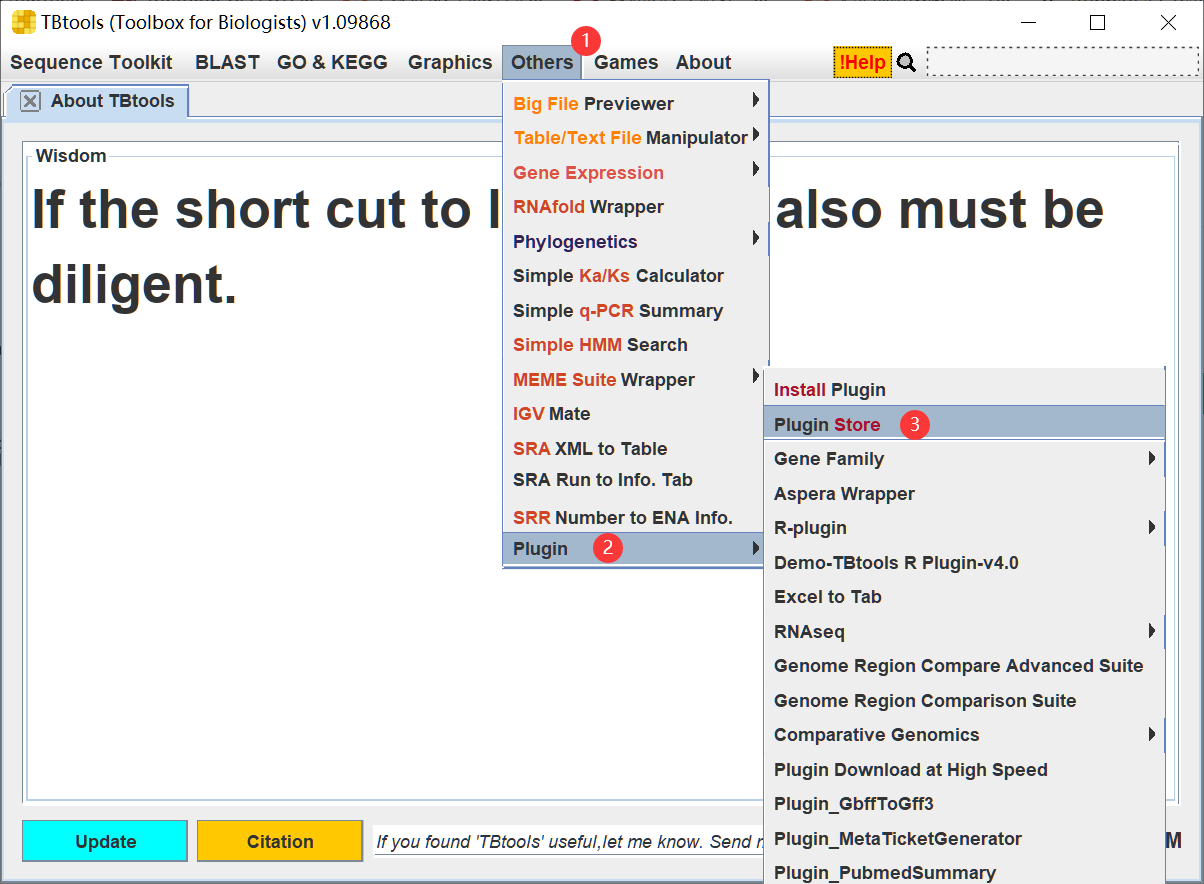
\includegraphics[width=0.8\textwidth]{./image/gdk/8.3.1.png}

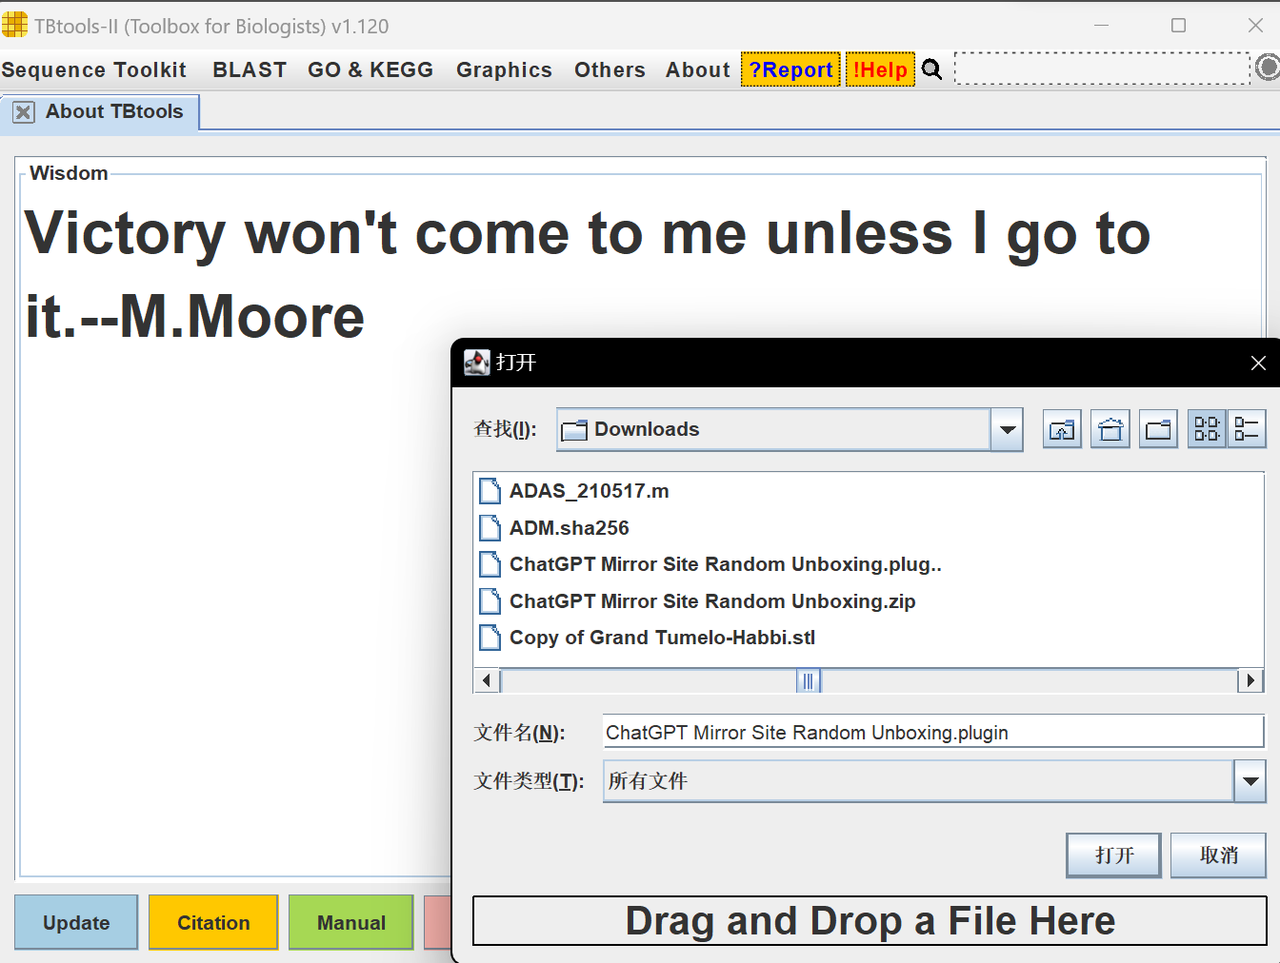
\includegraphics[width=0.8\textwidth]{./image/gdk/8.3.2.png}

安装完成后重启软件即可看见插件。

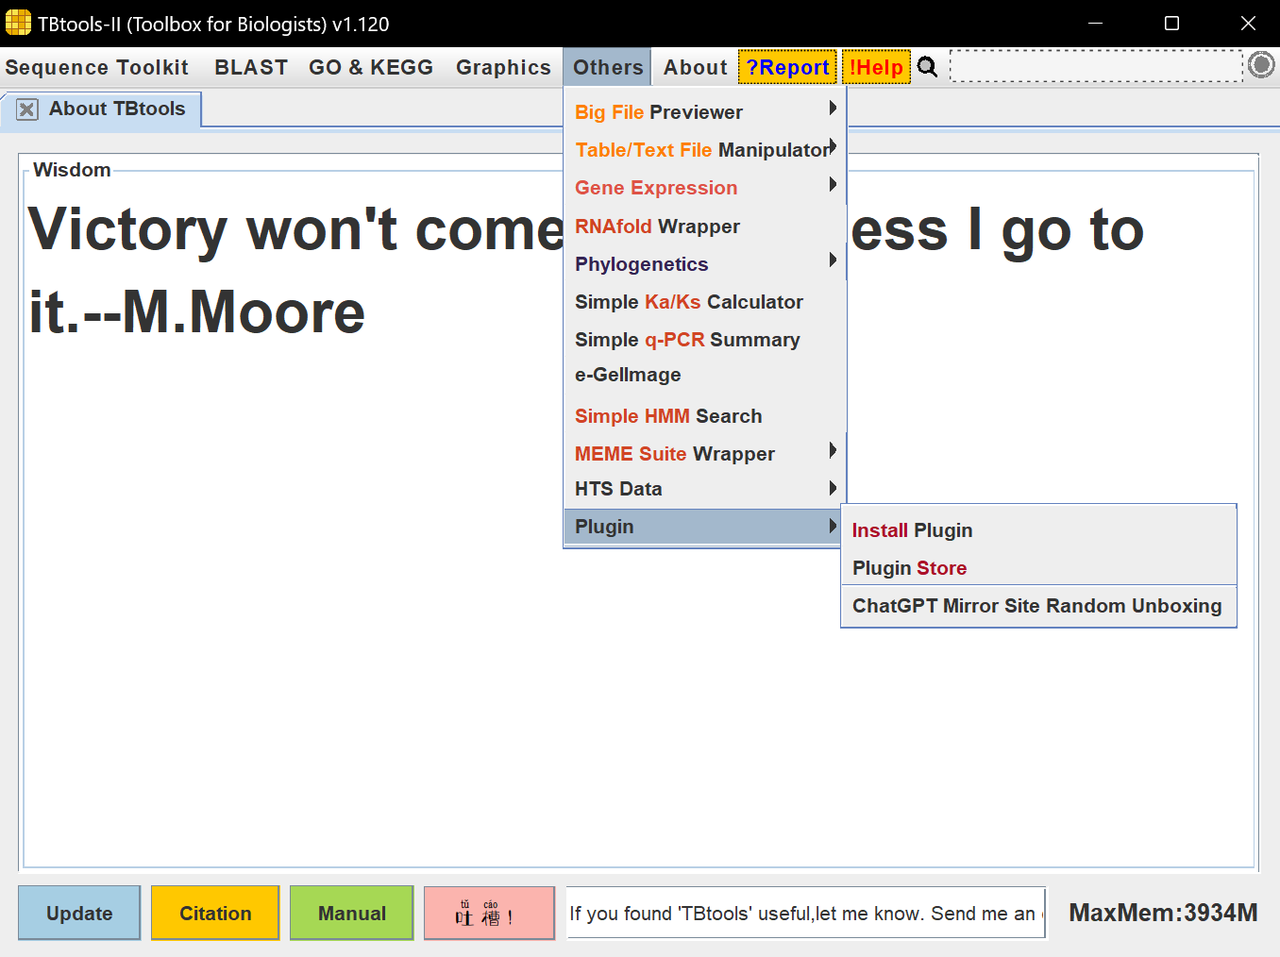
\includegraphics[width=0.8\textwidth]{./image/gdk/8.3.3.png}

\section*{参考资料}
\href{https://www.yuque.com/cjchen/hirv8i}{https://www.yuque.com/cjchen/hirv8i}

\href{https://zhuanlan.zhihu.com/p/144873860}{https://zhuanlan.zhihu.com/p/144873860}

\href{https://www.youtube.com/watch?v=O7\_w001f58c}{https://www.youtube.com/watch?v=O7\_w001f58c}